\chapter{Conclusion}
\label{sec:05-conclusion}

\epigraph{La dialectique est une machine amusante qui nous conduit /
  d'une manière banale / aux opinions que nous aurions eues en tout
  cas.}{\emph{Manifeste Dadá} (1918)\\\textsc{Tristan Tzara}}

This master's thesis project served, mainly, two purposes. First, to
recapitulate, rationalise and re-focus a long-term project that has
served its authors as learning sketchbook for many years. Second, to
give the first big steps in lifting the software to a professional
quality grade. Of course, there is a lot of work to be done. In the
analysis chapter the project was planned for a long-term development
in a iterative process. This allows us to concentrate on feasible
mid-term goals while building a broadly scoped system. Two of these
iterations have been successfully accomplished. 

Coming from a computer-science background, admittedly, we are still
quite amateur in many musical and even digital signal processing
aspects. Instead, we focused in what we can do better --- exploiting
programming languages abstraction facilities, making scalable
architectures and applying and eliciting design patterns in order to
write shorter, safer and faster code. The upcoming new C++ standard
provided us with a big open ground for research in new ways of using
multi-paradigm programming for our purpose. The most novel part of our
work is concentrated in our first iteration, where template
metaprogramming and concept-based design allowed us to write a sound
processing library that is generic yet efficient and safe. The last
stage also included relevant novelties --- like our polymorphic event
system for real-time processing --- yet being more pragmatical and
focused on requirement satisfaction and enabling future concrete
features, like a hierarchical patches, a plug-in system, and so on. We
should not, though, look at these advancements indulgently. Their own
chapters further discusses their benefits, caveats, and open issues
for improvement.

\begin{figure}[h!]
  \centering
  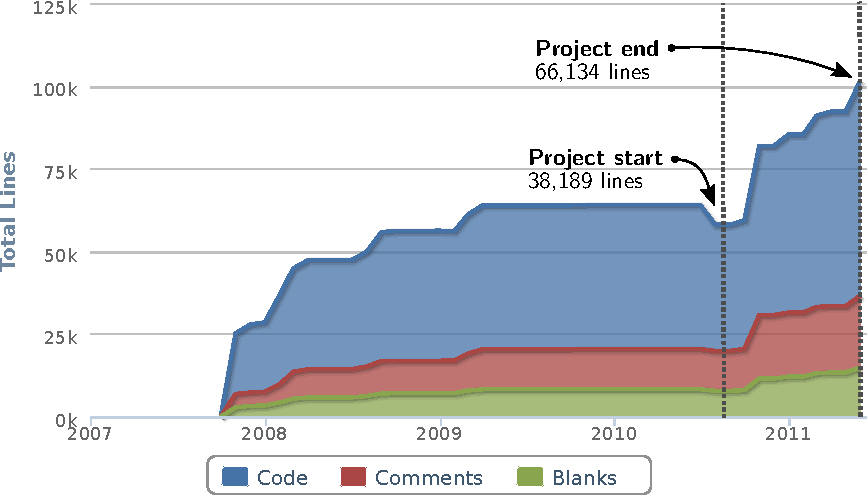
\includegraphics[width=\textwidth]{pic/dev-progress.pdf}
  \caption{Development progress in code lines.}
  \label{fig:dev-progress}
\end{figure}

Figure \ref{fig:dev-progress} shows the project growth in lines of
code, measured automatically from the sources repository by the Ohloh
webpage\footnote{Ohloh is a social network for Free Software
  development. Visit Psychosynth's page for further statistics:
  \url{https://www.ohloh.net/p/12930}}. Around 30000 new lines of code
have been added. Most of our work have involved refactoring --- in
other statistics, Ohloh states that around 100000 lines of code have
been changed during all the commits. This have been the biggest effort
since the participation of the project in the Free Software
Contest. Including \emph{``logic code only''} Ohloh estimates that the
total effort of the project --- since its beginning in mid 2007 --- in
12 person-years. It used the \emph{Basic COCOMO} \cite{bohem00cocomo}
method with coefficients $a = 2.4, b = 1.05$ to yield such result.

When looking into the future there are many possibilities. We are half
way to fulfil the long-term goals that were proposed in the first two
chapters. Apart from following our current plan blindfolded, there are
some developments that may makes re-plan part of our future work.

\begin{figure}[h!]
  \centering
  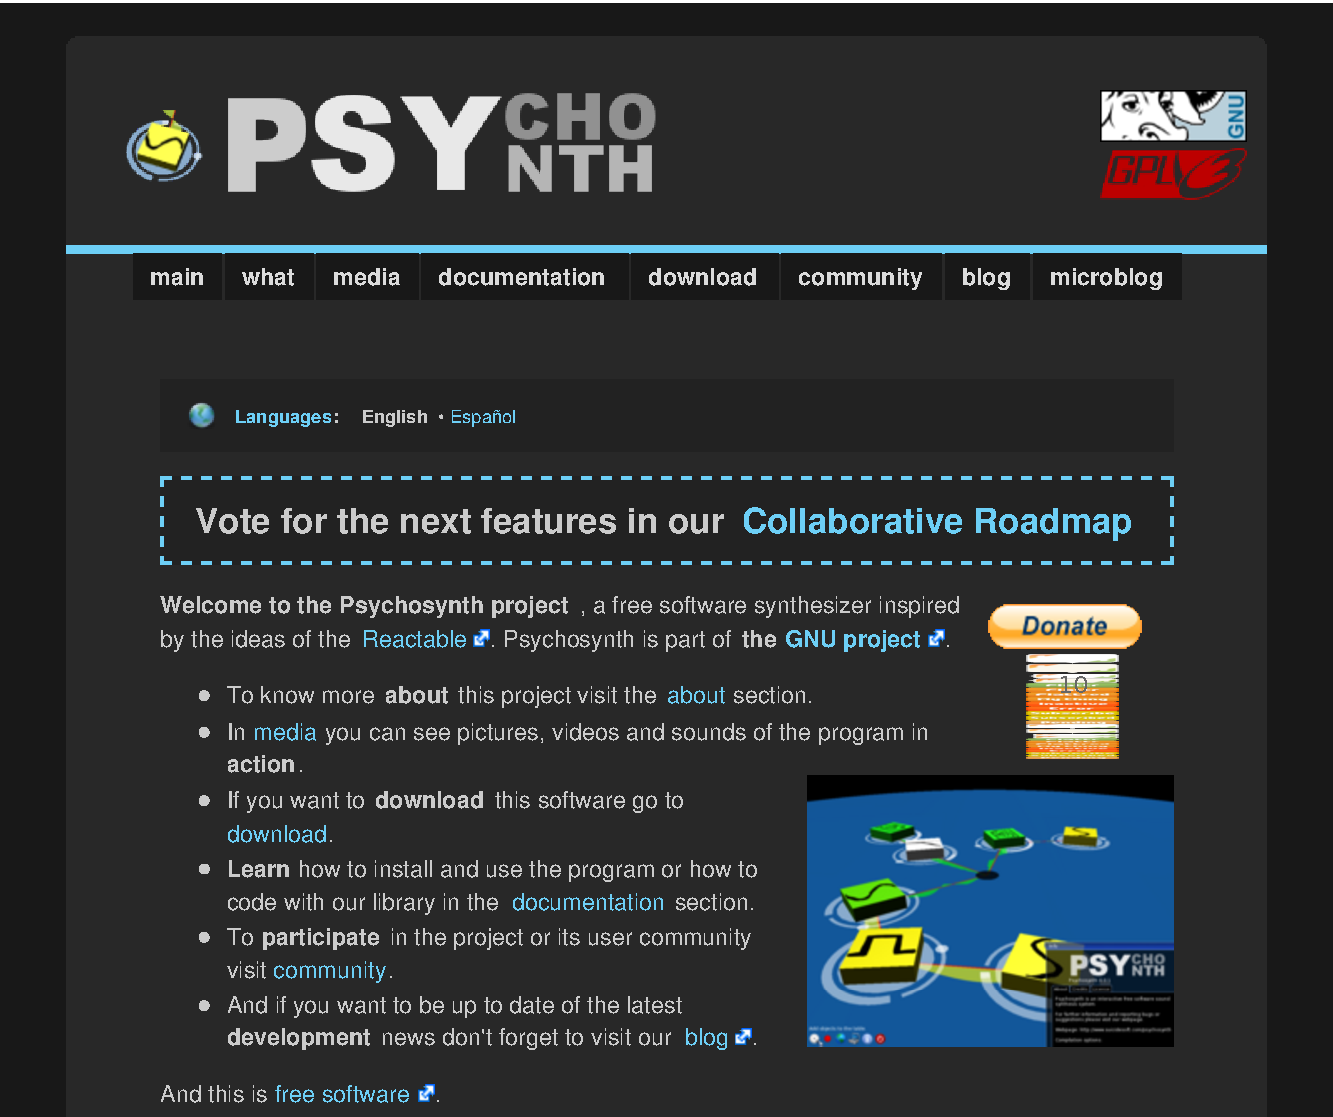
\includegraphics[width=\textwidth]{pic/webpage.pdf}
  \caption{GNU Psychosynth's new webpage design.}
  \label{fig:webpage}
\end{figure}

First, there is the \emph{Collaborative Roadmap}. As part of the
redesign of the project's web-page that we did in March (see figure
\ref{fig:webpage}) we included a feature request voting system based
on micro-donations. The Flattr\footnote{\url{http://flattr.com}}
social micro-payment network works as follows: each person puts some
money into his account each month. Then, different \emph{things} ---
music, software, pictures --- have a web button that users can press
to show support. At the end of the month, the money in someones'
account is distributed among all the creators of the things he
supported. Usually, each individual thing do not get much, but very
popular things can get a significant amount. Also, each Flattr button
has a counter with the number of people that pressed it. We use this
system in an special way: each potential feature not yet developed has
its own Flattr button. If someone thinks some feature is more urgent
than another, he can push for his opinion to be taken into account by
showing some commitment by making a micro-donation in this
system. Table \ref{tab:flattr} shows the current ranking in the
Collaborative Roadmap.

\begin{table}[h]
  \centering
  \begin{tabular}{r|l}
    Votes & Thing \\ \hline
    10 & GNU Psychosynth --- general \\
    5 & Audio input \\
    3 & MIDI support \\
    1 & Plug-in system \\
    1 & Tangible user interface \\
    1 & VST plug-ins \\
    & ...
  \end{tabular}
  \caption{Current ranking in the \emph{Collaborative Roadmap}, as in June 2010}
  \label{tab:flattr}
\end{table}

The Collaborative Roadmap credibility depends on whether we actually
take it into account. Thus, now that this master's thesis project is
over, we will devote some time to the most voted items. Indeed, the
``Audio Input'' feature seems quite feasible and fun to have,
so... why not?

Moreover, the growing interest in the project are opening the doors
for quite interesting collaborations. The ArtQuimia Music Production
School\footnote{\url{http://www.artquimia.net/}} have been supporting
the project since we started our requirement elicitation a year ago,
and we are grateful for this. More recently, Miguel Vazquez-Prada
contacted us to join efforts in building experimental tangible
instruments. He has already built a ReacTable clone called
Tangiblex\footnote{\url{http://www.tangiblex.net/}} with impressive
results (figure \ref{fig:tangiblex}). Hopefully this is the beginning
of a very fruitful collaboration. Indeed, hardware-software pair is
probably one of the best ways to build a business model for a consumer
oriented application while respecting user's freedom with
non-privative licenses. Also, Intel is offering a wide range of grants
and other kinds of support and partnership to promote their Meego
platform and Atom-based devices. That might be a good chance to
prioritise a port for multi-touch devices --- a very interesting
development with open grounds for experimentation and innovation.

\begin{figure}[h!]
  \centering
  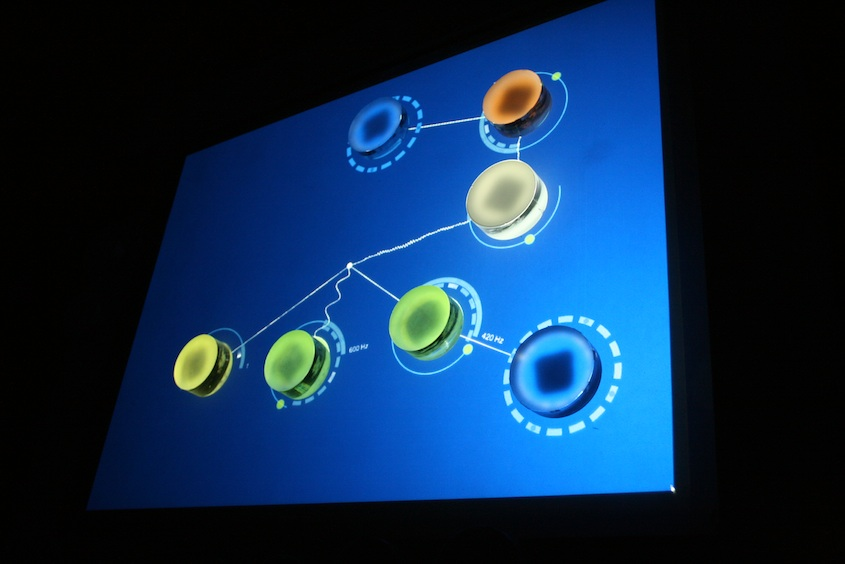
\includegraphics[width=\textwidth]{pic/fidumusic.jpg}
  \caption{The Tangiblex ReacTable-alike tangible instrument.}
  \label{fig:tangiblex}
\end{figure}

Anyway, whatever happens next, we have enjoyed and learnt a lot during
the development of this project. That is, indeed, all what one should
expect from a master's thesis project.

Thanks a lot for reading this document.

%%% Local Variables: 
%%% mode: latex
%%% TeX-master: "00-main"
%%% End: 
